% 隔離テスト用ドライバ: 反応器クラスタ 5-9 のみ単独ビルド（共有 main.tex に影響しない）
% 2026-06-07 リネーム後: 旧4-8 → 新5-9（熱統合が4に挿入されたため +1）
\documentclass[11pt,aspectratio=43,dvipsnames]{beamer}
\usepackage{luatexja}
\usepackage[match]{luatexja-fontspec}
\setmainjfont{HaranoAjiGothic}
\setsansjfont{HaranoAjiGothic}
\renewcommand{\kanjifamilydefault}{\gtdefault}
\usepackage{amsmath, amssymb}
\usepackage[version=4]{mhchem}
\usepackage{booktabs}
\usepackage{multirow}
\usepackage{colortbl}
\usepackage{graphicx}
\graphicspath{{figures/}}
\usepackage{pgfplots}
\pgfplotsset{compat=1.18}
% =====================================================================
%  seminar テーマ定義（既存 Marp デザインの Beamer 再現）
%  ・濃青の恒常ヘッダーバー（セクション名＋ページ番号）
%  ・専用表紙（アクセントライン＋グラデ背景）
%  ・本文は白地・濃青見出し
%  main.tex から \input する（パッケージではなく生プリアンブル）
% =====================================================================

% ---- ベース：装飾の少ないテーマから組む -----------------------------
\usetheme{default}
\usefonttheme{professionalfonts}
\setbeamertemplate{navigation symbols}{}   % ナビゲーション記号を消す

% ---- TikZ（ヘッダー・表紙・矢印などで使用）-------------------------
\usepackage{tikz}
\usetikzlibrary{arrows.meta, positioning, calc, shapes.geometric, fit, patterns}

% ---- 配色（ルール準拠）---------------------------------------------
\definecolor{HeaderBlue}{HTML}{0f5a7a}   % ヘッダー・見出しの濃青
\definecolor{DateGray}{HTML}{334b5e}     % 表紙の日付グレー
\definecolor{TitleBG}{HTML}{edf5fb}      % 表紙グラデの薄青

% コンテンツ用パレット（図・ハイライト・矢印で共通利用）
\definecolor{ArrowBlue}{HTML}{1F6FC4}    % 矢印・強調の青
\definecolor{HiPink}{HTML}{F4B6BE}       % ハイライト見出し（暖色）
\definecolor{HiBlue}{HTML}{C7DCEF}       % ハイライト見出し（寒色）
\definecolor{IpaBlue}{HTML}{1F5FC4}      % グラフ系列1（青）
\definecolor{DipeOrange}{HTML}{E8821E}   % グラフ系列2（橙）
\definecolor{SpRed}{HTML}{C0392B}        % 反応式：プロピレン強調の赤
\definecolor{SpBlue}{HTML}{1F6FC4}       % 反応式：エテン・エタン・CH0.5 の青

% 帯（ヘッダーバー）のパート別配色（寒色グラデ）。本文枠線は HeaderBlue のまま。
%  1-4 導入・全体像／5-9 反応・反応器／10-13 分離／14-17 最適化・経済・結言
\definecolor{barA}{HTML}{0F5A7A}   % 1-4  青緑
\definecolor{barB}{HTML}{1D6E6E}   % 5-9  シアン寄り
\definecolor{barC}{HTML}{2E4C8A}   % 10-13 青
\definecolor{barD}{HTML}{4A3C84}   % 14-17 紫

\setbeamercolor{normal text}{fg=black, bg=white}
\setbeamercolor{frametitle}{fg=HeaderBlue, bg=white}
\setbeamercolor{itemize item}{fg=HeaderBlue}
\setbeamercolor{itemize subitem}{fg=HeaderBlue}
\setbeamercolor{block title}{fg=white, bg=HeaderBlue}
\setbeamercolor{block body}{fg=black, bg=TitleBG}
\setbeamercolor{alerted text}{fg=HeaderBlue}

% ---- フォントサイズ（Marp px をおおよそ pt に対応）------------------
\setbeamerfont{frametitle}{size=\large, series=\bfseries}   % スライド見出し ~44px

% ---- 恒常ヘッダーバー（headline）-----------------------------------
%  左：セクション名（無ければロゴ枠）／右：ページ番号
\newcommand{\HeaderLogo}{}   % ロゴを入れるなら \renewcommand で画像指定
% 本線の総枚数（分母）。appendix に入ると分子がこれを超え、本線/付録を見分けられる。
\newcommand{\MainTotal}{17}
% パート別に帯色を選ぶ：1-4=barA／5-9=barB／10-13=barC／14-17=barD。
% スライド4の独自帯（CC・GCC）など headline を上書きする箇所でも呼べるよう独立コマンド化。
% 併せて本文アクセント色 HeaderBlue 自体をそのパート色へ再定義し、各スライドの
% 図・枠線・矢印・ボックス（HeaderBlue 参照）をパート色に連動させる（\colorlet は大域的）。
% headline はフレーム本文より前に組まれるため、ここでの再定義が本文に効く。
\newcommand{\SetBarColor}{%
  \ifnum\insertframenumber<5\setbeamercolor{headerbar}{fg=white, bg=barA}\colorlet{HeaderBlue}{barA}%
  \else\ifnum\insertframenumber<10\setbeamercolor{headerbar}{fg=white, bg=barB}\colorlet{HeaderBlue}{barB}%
  \else\ifnum\insertframenumber<14\setbeamercolor{headerbar}{fg=white, bg=barC}\colorlet{HeaderBlue}{barC}%
  \else\setbeamercolor{headerbar}{fg=white, bg=barD}\colorlet{HeaderBlue}{barD}%
  \fi\fi\fi}
\setbeamertemplate{headline}{%
  \ifnum\insertframenumber>0\relax
    \SetBarColor
    \begin{beamercolorbox}[wd=\paperwidth, ht=4.5ex, dp=1.8ex,
                           leftskip=1.2em, rightskip=1.2em]{headerbar}%
      \color{white}\bfseries\large
      \insertsectionhead%
      \hfill
      \insertframenumber/\MainTotal%
    \end{beamercolorbox}%
  \fi
}
\setbeamercolor{headerbar}{fg=white, bg=barA}
\setbeamertemplate{footline}{}             % フッターは使わない
\setbeamersize{text margin left=3mm, text margin right=3mm}  % 本文を横幅ぎりぎりまで

% 【必須ルール】帯と本文の間の余白を詰める（全スライド共通）。
%  beamer 既定の天井スキップで本文が帯から離れるのを、headline 直後の負スキップで打ち消す。
%  情報量最優先：無駄な上余白は作らない。各スライドは [t] 推奨。
\addtobeamertemplate{headline}{}{\vskip-2.6ex}

% frametitle はバーの直下に置く（左寄せ・濃青・太字）
\setbeamertemplate{frametitle}{%
  \vskip0.6ex
  \hspace{0.6em}\usebeamerfont{frametitle}\usebeamercolor[fg]{frametitle}\insertframetitle\par
  \vskip0.2ex
}

% ---- 箇条書きをシンプルに ------------------------------------------
\setbeamertemplate{itemize item}{\textbullet}
\setbeamertemplate{itemize subitem}{--}

% =====================================================================
%  再利用ヘルパー（どのスライドでも使える共通部品）
% =====================================================================
% 青い矢印 →（行中に置ける。結論や対応関係の明示に）
\newcommand{\bluearrow}{\tikz[baseline=-0.5ex]\draw[ArrowBlue, line width=1pt,
  -{Stealth[length=2.2mm]}] (0,0)--(0.55,0);}

% ハイライト見出し  \hilite{色}{テキスト}  例: \hilite{HiPink}{IPA選択率の温度依存性}
\newcommand{\hilite}[2]{\colorbox{#1}{\bfseries\normalsize #2}}

% パラメータ表  \paramtable{ 項目 & 値 \\ ... }  （左:項目 右:値、単位は数式推奨）
\newcommand{\paramtable}[1]{%
  {\footnotesize\renewcommand{\arraystretch}{1.15}%
   \begin{tabular}{@{\hspace{1em}}ll@{}}#1\end{tabular}}}

% =====================================================================
%  専用表紙コマンド  \seminartitlepage
%  ルール準拠：アクセントライン(120x8px相当) + 160度グラデ背景
%               h1 60px / h2 34px濃青 / 著者27px / 日付22pxグレー
%  使い方: \title{} \subtitle{} \author{} \date{} を設定後に呼ぶ
% =====================================================================
\newcommand{\seminartitlepage}{%
  \begin{frame}[plain]
    \begin{tikzpicture}[remember picture, overlay]
      % 背景グラデ（左上 薄青 → 右下 白、斜め）
      \shade[top color=TitleBG, bottom color=white, shading angle=20]
        (current page.south west) rectangle (current page.north east);
      % アクセントライン（上から少し下げて左に）
      \fill[HeaderBlue]
        ([xshift=9mm, yshift=-12mm]current page.north west)
        rectangle ++(16mm, 1.1mm);
      % テキストブロック（左寄せ・縦中央付近）
      \node[anchor=center, text width=0.86\paperwidth, align=center]
            at (current page.center) {%
        {\fontsize{22pt}{28pt}\selectfont\bfseries\color{black}\inserttitle\par}
        \vspace{0.3em}
        {\fontsize{16pt}{20pt}\selectfont\bfseries\color{HeaderBlue}\insertsubtitle\par}
        \vspace{1.0em}
        {\fontsize{13pt}{17pt}\selectfont\color{black}\insertauthor\par}
        \vspace{0.4em}
        {\fontsize{11pt}{14pt}\selectfont\color{DateGray}\insertdate\par}
      };
    \end{tikzpicture}
  \end{frame}
}

\setlength{\overfullrule}{6pt}
\begin{document}
\setcounter{framenumber}{4}
\section{反応工程}% =====================================================================
%  04  反応工程 — 反応ネットワーク・速度式・触媒失活
%  source_memo: 04_reaction.tex §4.2(反応ネットワークと速度式) /
%               §4.3.2-3(コーキングと活性低下 a(t,T))
%  失活グラフ実データ: pdh_simulator/src/catalyst_model.py _A_MATRIX
%               （要項§3-3 提供データ、温度400-700C × 時間0-30min）
%  方針：反応器モデル（支配方程式・Ergun）は載せない。
%        上=反応式と速度式／下左=触媒失活の要点／下右=a(t,T) グラフ。
%        色は反応式の化学種と、温度で意味を持つグラフの系列のみ。
% =====================================================================
% 活性 a を緑の太字で統一表示するマクロ
\definecolor{ActGreen}{HTML}{1BC24A}
\providecommand{\actA}{}\renewcommand{\actA}{{\color{ActGreen}\scalebox{1.2}{\ensuremath{\boldsymbol{a}}}}}
% 左カラム「触媒失活」見出し＋説明文を丸ごと左右に動かすつまみ。
% 正で右へ・負で左へ（0 で本文左マージン3mmのまま）。見出しと本文は連動して動く。ここの数字だけ変える。
\newlength{\descIndent}\setlength{\descIndent}{-2.8mm}
% 説明文の箱の幅。広げるほどグラフ左の余白を文章が使い、折り返しが減る。
\newlength{\descWidth}\setlength{\descWidth}{46mm}
% グラフ横幅を左から縮める量。大きいほどグラフが小さくなり、文章の余地が増える（右枠はスライド端のまま）。
\newlength{\grShrink}\setlength{\grShrink}{6mm}
\begin{frame}[t]

  \vspace*{0.6em}
  % ===== 上：反応ネットワーク + 速度式（全幅）======================
  {\normalsize
   \renewcommand{\arraystretch}{1.18}%
   \begin{tabular}{@{}l@{\hspace{0.7em}}l@{\hspace{0.6em}}l@{}}
     {\scriptsize 脱水素}
       & \setlength{\fboxsep}{4pt}\setlength{\fboxrule}{1.2pt}%
         \fcolorbox{HeaderBlue}{white}{\boldmath$\mathrm{C_3H_8 \rightleftharpoons {\color{SpRed}C_3H_6} + H_2}$}
       & $\displaystyle r_1 = \actA\,k_1\frac{p_{\mathrm{C_3H_8}} - p_{\mathrm{C_3H_6}}p_{\mathrm{H_2}}/K_{\mathrm{eq}}}{1 + p_{\mathrm{C_3H_6}}/K_B}$ \\
     {\scriptsize クラッキング} & {\boldmath$\mathrm{C_3H_8 \rightarrow {\color{SpBlue}C_2H_4} + CH_4}$}
       & $\displaystyle r_2 = k_2\,p_{\mathrm{C_3H_8}}$ \\
     {\scriptsize 水素化} & {\boldmath$\mathrm{{\color{SpBlue}C_2H_4} + H_2 \rightarrow {\color{SpBlue}C_2H_6}}$}
       & $\displaystyle r_3 = k_3\,p_{\mathrm{C_2H_4}}p_{\mathrm{H_2}}$ \\
     {\scriptsize コーキング} & {\boldmath$\mathrm{{\color{SpRed}C_3H_6} \rightarrow 3\,{\color{SpBlue}CH_{0.5}} + 2.25\,H_2}$}
       & {\scriptsize 物質収支では微量・触媒を失活} \\
   \end{tabular}}

  \vspace{0.12em}
  {\setlength{\fboxsep}{4pt}\setlength{\fboxrule}{0.8pt}%
   \noindent\fcolorbox{HeaderBlue}{white}{%
    \parbox{\dimexpr\linewidth-2\fboxsep-2\fboxrule\relax}{%
      \scriptsize 想定触媒：\textbf{\ce{Cr2O3}-\ce{Al2O3}}、主反応 \(\Delta H^{\circ}_{1}\approx +124\,\mathrm{kJ/mol}\)（吸熱）\par
      \vspace{2pt}
      速度定数は修正アレニウス、基準 $T_0=793\,\mathrm{K}$。$K_B$ はプロピレン吸着で高転化時 $r_1$ を抑制。}}}

  \vspace{0.35em}

  % ===== 下：触媒失活（左・簡潔）と a(t,T) グラフ（右・最大化）====
  %  方針：xラベルを yshift で目盛に密着、図タイトル・出典を負 vspace で詰めて
  %        運転時間の前後・タイトル/出典間の余白を最小化し、グラフ高さを最大化。
  \begin{columns}[T,onlytextwidth]
    \begin{column}{0.26\textwidth}
      \noindent\hspace*{\descIndent}\makebox[0pt][l]{\begin{minipage}[t]{\descWidth}
      \vspace*{1.0em}
      {\bfseries 触媒失活}\par
      \vspace{0.5em}
      {\footnotesize\raggedright\linespread{1.18}\selectfont
        コークが活性点を被覆し失活。\par
        \vspace{0.25em}
        活性 $\actA(t,T)$ は主反応 $r_1$ のみに作用\\
        （副反応には不作用）。\par
        \vspace{0.25em}
        運転温度では数分で大きく低下\par
        \quad $\to$\,\textbf{短周期の再生が不可欠}
      }
      \end{minipage}}
    \end{column}
    \begin{column}{0.74\textwidth}
      \noindent\hspace*{\dimexpr5.90mm+\grShrink\relax}\makebox[0pt][l]{%
      \begin{tikzpicture}
        \begin{axis}[
          font=\scriptsize,
          width=\dimexpr\linewidth-\grShrink\relax, height=5.08cm,
          xmin=0, xmax=30, ymin=0, ymax=1,
          enlarge x limits=false, enlarge y limits=false,
          xtick={0,10,20,30}, ytick={0,0.2,0.4,0.6,0.8,1.0},
          xlabel={運転時間 [min]}, ylabel={活性 $\actA$},
          xlabel near ticks, ylabel near ticks,
          x label style={yshift=2.55mm}, y label style={xshift=1.6mm},
          tick align=inside, xtick pos=both, ytick pos=both,
          legend style={font=\scriptsize, at={(0.985,0.98)}, anchor=north east,
                        draw=none, fill=white, fill opacity=0.7, text opacity=1,
                        inner sep=2pt, row sep=0.4pt},
          legend columns=1, legend cell align=left,
          no markers, line width=0.9pt,
        ]
          \addplot[blue]          coordinates {(0,1)(5,0.94)(10,0.90)(15,0.86)(20,0.84)(25,0.82)(30,0.81)}; \addlegendentry{$400\,^\circ$C}
          \addplot[cyan!70!blue]  coordinates {(0,1)(5,0.87)(10,0.80)(15,0.76)(20,0.72)(25,0.70)(30,0.68)}; \addlegendentry{$450\,^\circ$C}
          \addplot[teal]          coordinates {(0,1)(5,0.80)(10,0.68)(15,0.622)(20,0.57)(25,0.52)(30,0.49)}; \addlegendentry{$500\,^\circ$C}
          \addplot[olive]         coordinates {(0,1)(5,0.67)(10,0.52)(15,0.42)(20,0.36)(25,0.31)(30,0.28)}; \addlegendentry{$550\,^\circ$C}
          \addplot[orange]        coordinates {(0,1)(5,0.52)(10,0.35)(15,0.24)(20,0.18)(25,0.15)(30,0.13)}; \addlegendentry{$600\,^\circ$C}
          \addplot[red!70!black]  coordinates {(0,1)(5,0.38)(10,0.21)(15,0.13)(20,0.09)(25,0.07)(30,0.06)}; \addlegendentry{$650\,^\circ$C}
          \addplot[red]           coordinates {(0,1)(5,0.25)(10,0.12)(15,0.08)(20,0.06)(25,0.05)(30,0.04)}; \addlegendentry{$700\,^\circ$C}
          \node[font=\scriptsize\bfseries, anchor=north, fill=white, fill opacity=0.6,
                text opacity=1, inner sep=1.5pt] at (axis cs:10.5,0.985) {高温ほど急速に失活};
        \end{axis}
      \end{tikzpicture}}\par
      \centering
      \vspace*{-0.92em}
      {\scriptsize 　　　　　触媒活性 $\actA$ の経時低下（温度別）}\par
      \vspace*{-0.66em}
      {\tiny 速度式パラメータ・活性データの出典：第17回プロセスデザイン学生コンテスト要項}
    \end{column}
  \end{columns}

\end{frame}

\section{反応器設計}% =====================================================================
%  06  反応器設計 — 左右2カラム
%  左：性質→部品マップ（上）＋形式選定3判断の表（下）
%  右：反応器の説明文（上・小さめ）＋浅床軸流・多基切替式固定床の模式図（下）
%  source_memo: report/chapters/04_reaction.tex §4.1 形式選定3判断 /
%               §4.4 接触時間 τ∝1/u² / 反応器概念断面 TikZ。
%  方針：[t] で帯直下から少し下げる。丸括弧禁止。はみ出し・重なりなし。
% =====================================================================
\begin{frame}[t]

  \vspace{0.35em}
  \begin{columns}[T,onlytextwidth]
    % ===== 左：性質→部品マップ（上）＋形式選定の3判断の表（下）=====
    \begin{column}{0.40\textwidth}
      \centering
      \resizebox{\linewidth}{!}{%
      \begin{tikzpicture}[
        >=Stealth, font=\small,
        prop/.style={draw=black!50, rounded corners=2pt, align=center,
                     inner sep=3pt, minimum height=0.7cm, text width=2.0cm},
        part/.style={draw=HeaderBlue, fill=HiBlue!45, rounded corners=2pt, align=center,
                     inner sep=3pt, minimum height=0.6cm, text width=2.9cm,
                     font=\small\bfseries},
        link/.style={-{Stealth[length=2mm]}, ArrowBlue, line width=1pt},
      ]
        \node[prop] (heat) at (0,2.85) {吸熱};
        \node[prop] (eq)   at (0,1.42){平衡支配\\$0.5$ bar};
        \node[prop] (coke) at (0,0)   {コーキング\\数分で失活};
        \node[part] (hgm)   at (3.7,2.85) {床内 HGM 補温};
        \node[part] (shal)  at (3.7,1.9)  {浅床軸流};
        \node[part] (multi) at (3.7,0.95) {多基・大断面・低速};
        \node[part] (swing) at (3.7,0.0)  {切替式　反応 $\rightleftarrows$ 再生};
        \draw[link] (heat.east) -- (hgm.west);
        \draw[link] (eq.east)   -- (shal.west);
        \draw[link] (eq.east)   -- (multi.west);
        \draw[link] (coke.east) -- (swing.west);
      \end{tikzpicture}}\par

      \vspace{1.0em}
      \raggedright
      {\small\bfseries 形式選定の3判断と採用根拠}\par
      \vspace{0.4em}
      {\scriptsize\renewcommand{\arraystretch}{1.15}%
       \begin{tabular}{@{}l l c@{}}
         \toprule
         判断 & 候補 & 採否 \\
         \midrule
         \multirow{2}{*}{触媒再生}
            & 移動床            & $\times$ \\
            & {\color{SpRed}並列切替固定床} & $\bigcirc$ \\
         \midrule
         \multirow{3}{*}{流通形式}
            & 軸流深床   & $\times$ \\
            & 径方向流   & $\triangle$ \\
            & {\color{SpRed}浅床軸流}   & $\bigcirc$ \\
         \midrule
         \multirow{2}{*}{熱補償}
            & 段間再加熱 & $\times$ \\
            & {\color{SpRed}床内 HGM}   & $\bigcirc$ \\
         \bottomrule
       \end{tabular}}\par
      \vspace{0.25em}
      {\tiny\raggedright $\times$ 移動床は失活追従不可、$\triangle$ 径方向流は機構複雑\par
       \vspace{0.18em}
       $\times$ 段間再加熱は床温を戻すのみで分単位の急速失活に間に合わない。切替再生で蓄えた熱を HGM が床内補償\par}
    \end{column}

    % ===== 右：反応器の特徴（上・小さめ）＋模式図（下）============
    \begin{column}{0.60\textwidth}
      % 特徴文：左のフロー図から離すため右へインデント、文字は小さめ
      \hspace*{9mm}\begin{minipage}{\dimexpr\linewidth-9mm\relax}
        \raggedright
        {\bfseries 反応器の特徴}\par
        \vspace{0.3em}
        {\scriptsize\raggedright\linespread{1.18}\selectfont
          ・\textbf{Catofin 型}の浅床軸流・多基切替式固定床を採用。\par
          ・吸熱反応と再生（コーク燃焼）を周期的に切替え、\textbf{計 14 基}で連続運転。\par
          ・床内の蓄熱体 \textbf{HGM} が反応熱を供給し床温を維持。\par
          ・大断面・低流速で接触時間を確保（$\tau\propto 1/u^{2}$、流速半減で 4 倍）し、短周期切替で失活に追従。\par
        }
      \end{minipage}\par

      \vspace{1.2em}   % 模式図を下げ、最下部をスライド下端に合わせる
      \centering
      {\bfseries\color{SpRed}浅床軸流・多基切替式固定床の模式図}\par
      \vspace{0.15em}
      \resizebox{0.95\linewidth}{!}{%
      \begin{tikzpicture}[
        >=Stealth,
        proc/.style={-{Stealth[length=2.4mm]}, line width=1.2pt},
        wall/.style={line width=1.3pt},
        lead/.style={line width=0.4pt, black!55},
        lbl/.style={font=\large, align=center},
      ]
        \foreach \dx/\toplab/\botlab/\stt/\bcol/\acol in {%
           0/{原料ガス}/{製品}/{反応中}/{ArrowBlue}/{ArrowBlue},
           5.4/{空気}/{燃焼ガス}/{再生中}/{orange!85!red}/{orange!85!red}%
        }{
          \begin{scope}[xshift=\dx cm]
            \def\R{1.72}\def\Hb{1.48}\def\ry{0.80}
            \draw[wall] (-\R,0)--(-\R,\Hb); \draw[wall] (\R,0)--(\R,\Hb);
            \draw[wall] (-\R,\Hb) arc[start angle=180, end angle=0, x radius=\R, y radius=\ry];
            \draw[wall] (\R,0) arc[start angle=0, end angle=-180, x radius=\R, y radius=\ry];
            \draw[line width=0.7pt] (-\R+0.07,\Hb-0.30)--(\R-0.07,\Hb-0.30);
            \fill[pattern=dots, pattern color=\bcol] (-\R+0.07,\Hb-0.80) rectangle (\R-0.07,\Hb-0.38);
            \draw[black!40] (-\R+0.07,\Hb-0.80) rectangle (\R-0.07,\Hb-0.38);
            \draw[line width=0.7pt] (-\R+0.07,\Hb-0.86)--(\R-0.07,\Hb-0.86);
            \draw[wall] (-0.17,\Hb+\ry-0.02)--(-0.17,\Hb+\ry+0.30);
            \draw[wall] (0.17,\Hb+\ry-0.02)--(0.17,\Hb+\ry+0.30);
            \draw[proc, \acol] (0,\Hb+\ry+0.92)--(0,\Hb+\ry+0.36);
            \node[lbl, above] at (0,\Hb+\ry+0.90) {\toplab};
            \draw[wall] (-0.17,-\ry+0.02)--(-0.17,-\ry-0.30);
            \draw[wall] (0.17,-\ry+0.02)--(0.17,-\ry-0.30);
            \draw[proc, \acol] (0,-\ry-0.36)--(0,-\ry-0.92);
            \node[lbl, below] at (0,-\ry-0.90) {\botlab};
            \node[font=\Large\bfseries, text=\acol] at (0,-\ry-1.74) {\stt};
          \end{scope}
        }
        \node[lbl, anchor=east, font=\scriptsize] (bl) at (-2.15,1.30) {触媒・HGM\\浅床};
        \draw[lead] (bl.east) -- (-1.60,1.00);
        \node[lbl, anchor=east, font=\scriptsize] (gl) at (-2.15,0.40) {支持グリッド};
        \draw[lead] (gl.east) -- (-1.60,0.62);
        \draw[{Stealth[length=2.6mm]}-{Stealth[length=2.6mm]}, line width=1.6pt, ArrowBlue]
              (1.95,0.95) -- (3.45,0.95);
        \node[lbl, ArrowBlue, font=\normalsize\bfseries, align=center] at (2.7,1.55) {周期\\切替};
        \node[font=\large, align=center, text=black] at (2.7,-3.45)
              {反応 $\rightleftarrows$ 再生 を周期交代　計 14 基};
      \end{tikzpicture}}
    \end{column}
  \end{columns}

\end{frame}

\section{支配方程式}% =====================================================================
%  07  支配方程式（ヘッダー＝支配方程式）
%  source_memo: 04_reaction.tex §4.2.4 支配方程式（物質・エネルギー・Ergun）/
%               §4.2.5 スイング設計（N_swing,sets・V_cat・N_parallel・V_vessel）/
%               §4.2 量論行列(eq:stoich_matrix)・成分ベクトル
%  方針：見出しは小チップ。速度式は §反応工程で既出のため載せない。
%        各列に「式（上）＋記号表（下）」を縦積みし、中央を全高の縦線で仕切る。
%        左＝モデル（式＋記号表：ベクトル/行列 F・r・ν・ΔH・Cp を収録）。
%        右＝スイング設計（式＋記号表）。表は 1記号=1行・2群・群間に縦罫線。
%        モデル式は短いので左表を直下から始め余白を回収し表を最大化。色なし・丸括弧禁止。
% =====================================================================
\begin{frame}[t]

  \vspace{0.15em}

  \begin{columns}[T,onlytextwidth]
    % ===== 左：モデル（式＋記号表）================================
    \begin{column}{0.49\textwidth}
      \fbox{\scriptsize モデル}\par
      \vspace{0.75em}
      {\fontsize{5.5}{6.6}\selectfont [物質収支]}\par
      {\centering$\displaystyle\frac{d\boldsymbol{F}}{dz}=(1-\varepsilon)\,A_{\mathrm{cross}}\,\boldsymbol{\nu}\,\boldsymbol{r}$\par}
      \vspace{0.95em}
      {\fontsize{5.5}{6.6}\selectfont [エネルギー収支・断熱]}\par
      {\centering$\displaystyle\frac{dT}{dz}=-\frac{(1-\varepsilon)\,A_{\mathrm{cross}}\,\boldsymbol{\Delta H}^{\!\top}\boldsymbol{r}}{\boldsymbol{F}^{\!\top}\boldsymbol{C}_p}$\par}
      \vspace{0.95em}
      {\fontsize{5.5}{6.6}\selectfont [Ergun]}\par
      {\centering\resizebox{\linewidth}{!}{$\displaystyle\frac{dP}{dz}=-\Big[\,150\frac{(1-\varepsilon_b)^2\mu u}{\varepsilon_b^3(\phi d_p)^2}
           +1.75\frac{(1-\varepsilon_b)\rho u^2}{\varepsilon_b^3\phi d_p}\,\Big]$}\par}
      \vspace{0.6em}
      {\color{black!25}\rule{\linewidth}{0.4pt}}\par
      \vspace{0.45em}
      % --- 左表：モデルの記号（ベクトル/行列＋支配式スカラー）2群 ---
      \resizebox{\linewidth}{!}{%
       \renewcommand{\arraystretch}{1.25}%
       \begin{tabular}{@{}l l l @{\hspace{1em}}|@{\hspace{1em}} l l l@{}}
         \toprule
         $\boldsymbol{F}$        & モル流量 & mol/s
           & $\varepsilon_b$ & 粒子間空隙率 & -- \\
         $\boldsymbol{r}$        & 反応速度 & mol/m$^3$s
           & $d_p$          & 粒径          & m \\
         $\boldsymbol{\nu}$      & 量論行列 & --
           & $\phi$          & 形状係数      & -- \\
         $\boldsymbol{\Delta H}$ & 反応熱   & kJ/mol
           & $T$            & 温度          & K \\
         $\boldsymbol{C}_p$      & 熱容量   & J/molK
           & $P$            & 全圧          & Pa \\
         $z$                     & 軸位置   & m
           & $u$            & 空塔速度      & m/s \\
         $A_{\mathrm{cross}}$    & 断面積   & m$^2$
           & $\rho$          & 密度          & kg/m$^3$ \\
         $\varepsilon$           & 床/容器体積比 & --
           & $\mu$          & 粘度          & Pa$\cdot$s \\
         \bottomrule
       \end{tabular}}
    \end{column}

    % ===== 中央：全高の仕切り線 ==================================
    \begin{column}{0.02\textwidth}
      \centering
      {\color{black!35}\rule[-6.9cm]{0.6pt}{7.05cm}}
    \end{column}

    % ===== 右：スイング設計（式＋記号表）==========================
    \begin{column}{0.49\textwidth}
      \fbox{\scriptsize スイング設計}\par
      \vspace{0.45em}
      {\fontsize{5.5}{6.6}\selectfont [再生追従のセット数]}\par
      {\centering$\displaystyle N_{\mathrm{swing,sets}}=\left\lceil\frac{t_{\mathrm{regen}}}{t_{\mathrm{cyc}}}\right\rceil+1$\par}
      \vspace{0.35em}
      {\fontsize{5.5}{6.6}\selectfont [触媒体積]}\par
      {\centering$\displaystyle V_{\mathrm{cat}}=(1-\varepsilon)\,z_{\mathrm{cat}}\,\frac{\pi D^2}{4}$\par}
      \vspace{0.35em}
      {\fontsize{5.5}{6.6}\selectfont [容器分割の並列基数]}\par
      {\centering$\displaystyle N_{\mathrm{parallel}}=\max\!\left(\left\lceil\frac{V_{\mathrm{cat}}}{V_{\mathrm{cat,max}}}\right\rceil,\,1\right)$\par}
      \vspace{0.35em}
      {\fontsize{5.5}{6.6}\selectfont [容器1基の体積　CAPEX 基準]}\par
      {\centering$\displaystyle V_{\mathrm{vessel}}=\frac{z_{\mathrm{cat}}}{N_{\mathrm{parallel}}}\cdot\frac{\pi D^2}{4}$\par}
      \vspace{0.5em}
      {\color{black!25}\rule{\linewidth}{0.4pt}}\par
      \vspace{0.4em}
      % --- 右表：スイング設計の記号 2群 ---
      \resizebox{\linewidth}{!}{%
       \renewcommand{\arraystretch}{1.25}%
       \begin{tabular}{@{}l l l @{\hspace{1em}}|@{\hspace{1em}} l l l@{}}
         \toprule
         $z_{\mathrm{cat}}$   & 触媒層長 & m
           & $V_{\mathrm{cat}}$    & 触媒体積       & m$^3$ \\
         $D$                  & 内径     & m
           & $V_{\mathrm{vessel}}$ & 容器体積       & m$^3$ \\
         $t_{\mathrm{cyc}}$   & 反応時間 & s
           & $V_{\mathrm{cat,max}}$ & 最大触媒体積  & m$^3$ \\
         $t_{\mathrm{regen}}$ & 再生時間 & s
           & $N_{\mathrm{parallel}}$ & 並列基数     & -- \\
         & & & $N_{\mathrm{swing,sets}}$ & スイングセット数 & -- \\
         \bottomrule
       \end{tabular}}
    \end{column}
  \end{columns}

\end{frame}

\section{浅床軸流・多基スイング反応器}% =====================================================================
%  08  反応器プロファイル — 炉内 軸方向挙動＋検証諸元
%  source_memo: monitor/reactor_axial_profile.ipynb 出力
%               reactor_axial_TX.png / reactor_axial_selectivity.png、
%               §4.x 検証諸元 Table reactor_verification（trial #201）
%  方針：左=軸方向プロファイル2図（T/X のHGM補償効果・選択率の床内崩落）、
%        右=検証諸元。丸括弧禁止。
% =====================================================================
\begin{frame}

  \begin{columns}[T,onlytextwidth]
    % ===== 左：軸方向プロファイル =================================
    \begin{column}{0.6\textwidth}
      {\bfseries HGM 補償が床温を維持し転化率を伸ばす}\par
      \vspace{0.1em}
      \centering
      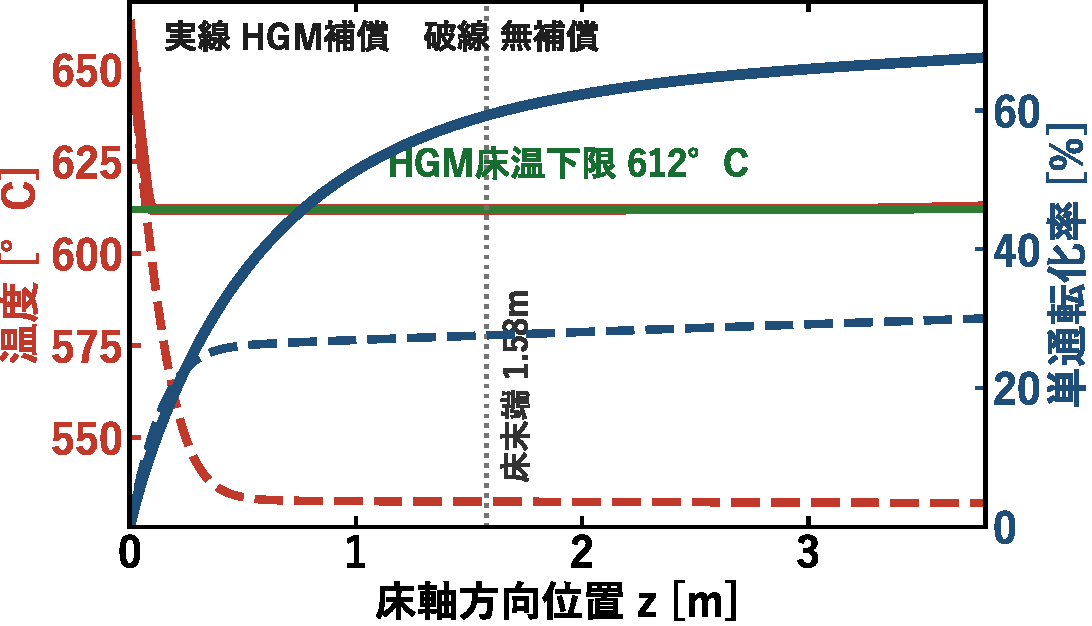
\includegraphics[width=0.78\linewidth]{reactor_axial_TX}\par
      \vspace{0.2em}
      {\bfseries 選択率は床後半で崩落し出口値へ収束}\par
      \vspace{0.1em}
      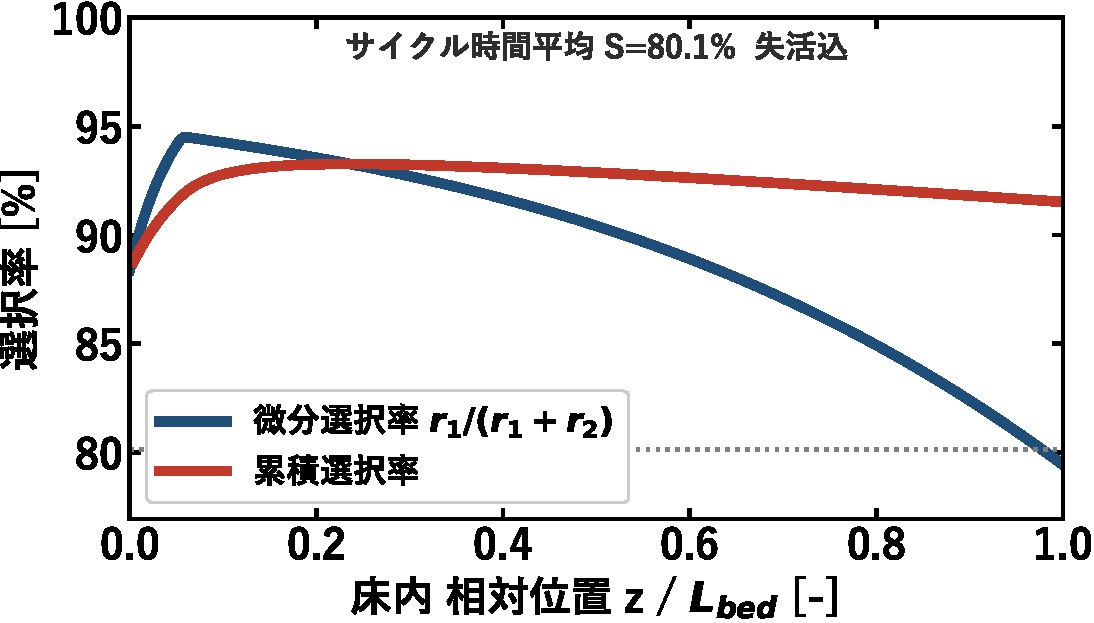
\includegraphics[width=0.78\linewidth]{reactor_axial_selectivity}\par
    \end{column}

    % ===== 右：検証諸元（trial #125）=============================
    \begin{column}{0.4\textwidth}
      {\bfseries 検証諸元　{\scriptsize 最良設計点}}\par
      \vspace{0.5em}
      {\setlength{\fboxsep}{5pt}\setlength{\fboxrule}{1pt}%
       \fcolorbox{HeaderBlue}{white}{%
        \footnotesize\renewcommand{\arraystretch}{1.25}%
        \begin{tabular}{@{}l@{\hspace{0.8em}}r@{}}
          入口温度 $T_{\mathrm{in}}$   & $935$ K \\
          出口温度 $T_{\mathrm{out}}$  & $885$ K \\
          床温降下 $\Delta T$          & $50$ K \\
          転化率 $X$                   & $40.6\,\%$ \\
          選択率 $S$                   & $80.1\,\%$ \\
          浅床厚 $L_{\mathrm{bed}}$    & $1.58$ m \\
          触媒粒径 $d_p$               & $5.84$ mm \\
          床 $\Delta P/P$              & $1.7\,\%$ \\
          総 $\Delta P/P$              & $3.3\,\%$ \\
          総基数 $N_{\mathrm{total}}$  & $14$ 基 \\
        \end{tabular}}}\par
      \vspace{0.8em}
      {\scriptsize 図の $T$・$X$ は新触媒断面、\par
       転化率 $40.6\,\%$・選択率 $80.1\,\%$ は\par
       失活を含むサイクル時間平均。\par
       無補償では床温が下限へ張り付き\par
       転化率が頭打ちとなる。}\par
    \end{column}
  \end{columns}

\end{frame}

\section{反応器分析}% =====================================================================
%  09  転化率の天井（断熱平衡）と熱補償 HGM・リサイクルの必然性（旧08、反応器プロファイルと順序入替）
%  ※ ヘッダーは main.tex の \section{転化率の天井} で設定。
%  source_memo: 04_reaction.tex §4.6 単通転化率と選択率の上限（断熱平衡の天井）/
%               §4.7 反応熱の補償方式（HGM）。図 reactor_xt_slide（figures/make_reactor_xt_slide.py）。
%               数値：ΔH1≈+124 kJ/mol、断熱平衡 524℃・23%、等温保持 78%、Q_HGM=24.96 MW（trial #201）。
%  方針：8(プロファイル)の後に「なぜHGMが要るか」を置く。
%        左＝問題（断熱の頭打ち）→打破（HGM→接触時間→リサイクル）、右＝X–T線図。
%        丸括弧禁止・色は天井の数値のみ赤。
% =====================================================================
\begin{frame}[t]

  \vspace{0.2em}

  \begin{columns}[T,onlytextwidth]
    % ===== 左：三段でまとめる（転化率の天井／打破＝多段 vs HGM／選択率の天井）===
    \begin{column}{0.53\textwidth}
      {\bfseries 転化率の天井}\par
      \vspace{0.35em}
      {\footnotesize
       ・強吸熱の自己冷却で断熱平衡に頭打ち\par
       \hspace{1em}断熱 {\color{SpRed}\textbf{23\,\%}}　$\Leftrightarrow$　等温保持 78\,\%\par
       ・触媒を増やしても破れない　律速は平衡\par
      }
      \vspace{1.0em}
      {\bfseries 天井の打破は二択}\par
      \vspace{0.35em}
      {\footnotesize
       ・多段直列＋段間再加熱で各段の平衡をリセット\par
       \hspace{1em}この方式は反応器が \textbf{3〜4 段}になる\par
       ・本設計は床内 HGM で床温維持・段間炉なし\par
       \hspace{1em}$\to$ 律速が接触時間へ　低速・多基で稼ぐ\par
       \hspace{1em}維持温度の平衡が上限 $\to$ \textbf{リサイクル必須}\par
      }
      \vspace{1.0em}
      {\bfseries 選択率の天井}\par
      \vspace{0.35em}
      {\footnotesize
       ・平衡近傍で微分選択率が崩落 $\to$ 積分 {\color{SpRed}\textbf{約 80\,\%}}\par
       ・固有上限 $S_{\max}=k_1/(k_1+k_2)$ は温度のみ\par
       \hspace{1em}$520\,^\circ$C で $99$\,\% ／ $750\,^\circ$C で $77$\,\%\par
      }
    \end{column}

    % ===== 右：断熱 X–T 線図（縦中央寄せ・キャプション無し）======
    \begin{column}{0.46\textwidth}
      \centering
      \vspace{2.8em}
      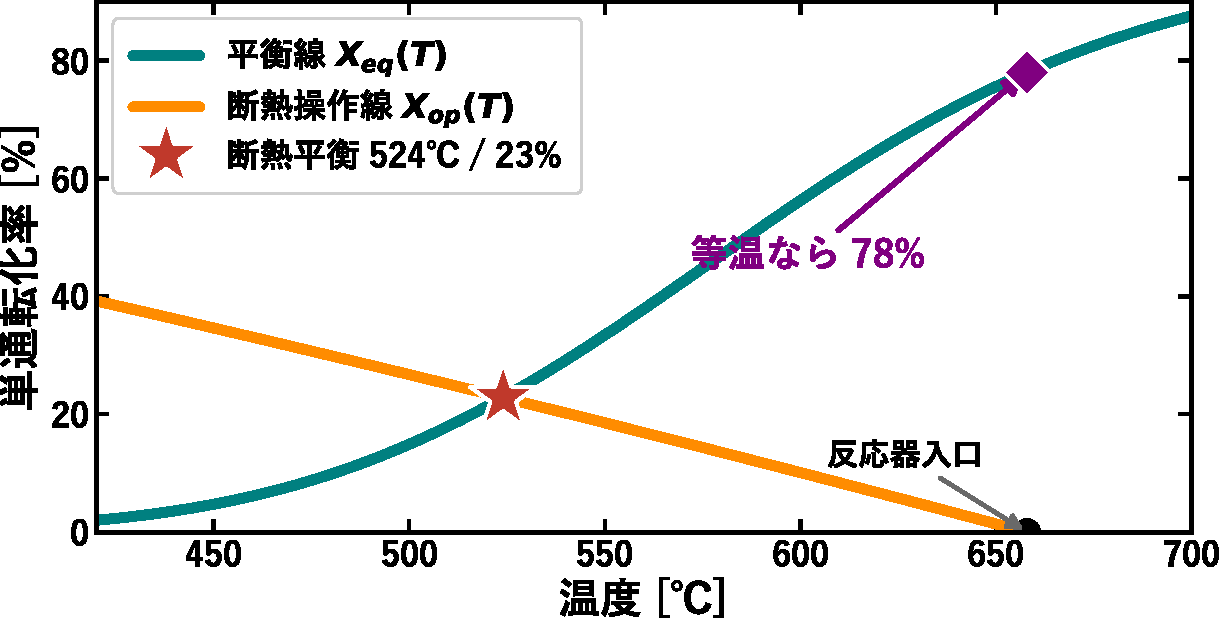
\includegraphics[width=\linewidth]{reactor_xt_slide}\par
    \end{column}
  \end{columns}

\end{frame}

\end{document}
